\subsection{Упражнение 1}

Создайте треугольный сигнал и напечатайте его. Примените diff к сигналу и напечатайте результат. Вычислите спектр треугольного сигнала, примените differentiate и напечатайте результат. Преобразуйте спектр обратно в сигнал и напечатайте его. Есть ли различия в воздействии diff и differentiate на этот сигнал?

\begin{lstlisting}[language=Python]
from thinkdsp import TriangleSignal

wave = TriangleSignal(freq=440).make_wave(duration=0.01, framerate=44100)
wave.plot()
decorate(xlabel='Time (s)')
\end{lstlisting}
\begin{figure}[H]
	\begin{center}
		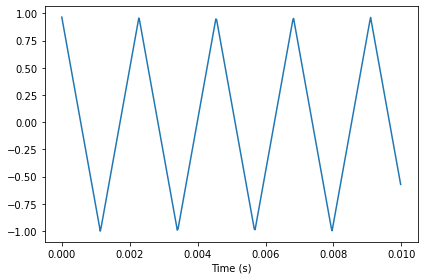
\includegraphics[scale=1]{fig/lab09/lab09_1.png}
		\caption{График треугольного сигнала}
	\end{center}
\end{figure}

\begin{lstlisting}[language=Python]
diff_wave = wave.diff()
diff_wave.plot()
decorate(xlabel='Time (s)')
\end{lstlisting}
\begin{figure}[H]
	\begin{center}
		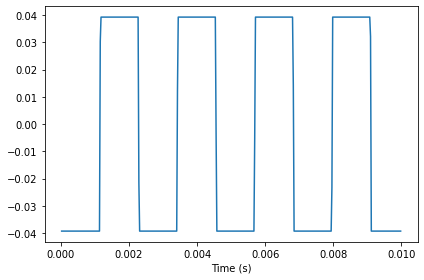
\includegraphics[scale=1]{fig/lab09/lab09_2.png}
		\caption{Сигнал после применения diff}
	\end{center}
\end{figure}

Получился прямоугольны сигнал с такой же частотой

\begin{lstlisting}[language=Python]
differentiate_wave = wave.make_spectrum().differentiate().make_wave()
differentiate_wave.plot()
decorate(xlabel='Time (s)')
\end{lstlisting}
\begin{figure}[H]
	\begin{center}
		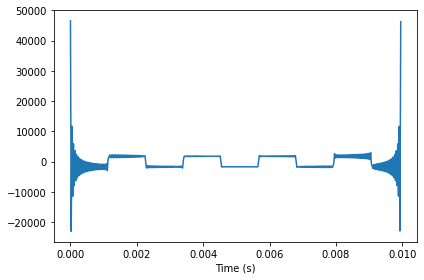
\includegraphics[scale=1]{fig/lab09/lab09_3.png}
		\caption{Сигнал после применения differentiate}
	\end{center}
\end{figure}

Вначале и в конце шум, вероятнее всего это связано c тем, что невозможно вычислить производную.

\subsection{Упражнение 2}

Создайте прямоугольный сигнал и напечатайте его. Примените cumsum и напечатайте результат. Вычислите спектр прямогоульного сигнала, примените integrate и напечатайте результат. Преобразуйте спектр обратно в сигнал и напечайте его. Есть различия в воздействии cumsum и integrate на этот сигнал?

Изучим влияние cumsum и integrate на прямоугольный сигнал.

\begin{lstlisting}[language=Python]
from thinkdsp import SquareSignal

wave = SquareSignal(freq=100).make_wave(duration=0.1, framerate=44100)
wave.plot()
decorate(xlabel='Time (s)')
\end{lstlisting}
\begin{figure}[H]
	\begin{center}
		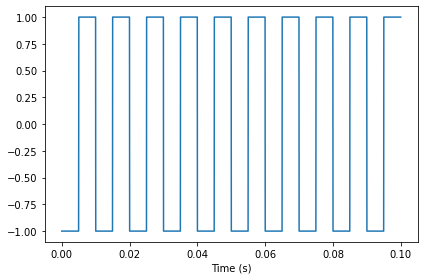
\includegraphics[scale=1]{fig/lab09/lab09_4.png}
		\caption{Рассматриваемый сигнал}
	\end{center}
\end{figure}

Применим cumsum:

\begin{lstlisting}[language=Python]
cumsum_wave = wave.cumsum()
cumsum_wave.plot()
decorate(xlabel='Time (s)')
\end{lstlisting}
\begin{figure}[H]
	\begin{center}
		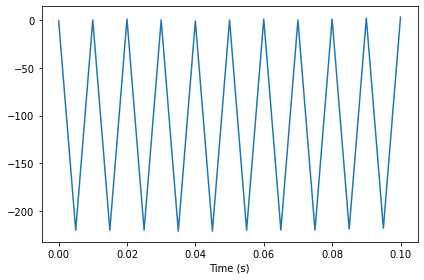
\includegraphics[scale=1]{fig/lab09/lab09_5.png}
		\caption{Рассматриваемый сигнал после применения cumsum}
	\end{center}
\end{figure}

Получился треугольный сигнал

Теперь интеграл спектра:

\begin{lstlisting}[language=Python]
int_spec = wave.make_spectrum().integrate()
int_spec.hs[0] = 0
int_wave = int_spec.make_wave()
int_wave.plot()
decorate(xlabel='Time (s)')
\end{lstlisting}
\begin{figure}[H]
	\begin{center}
		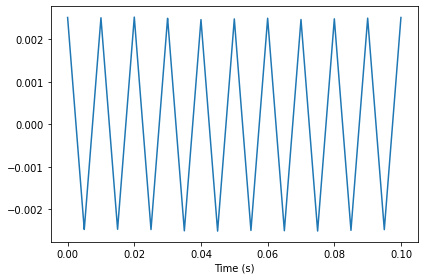
\includegraphics[scale=1]{fig/lab09/lab09_6.png}
		\caption{Рассматриваемый сигнал после применения integrate}
	\end{center}
\end{figure}

Спектральный интеграл также получлся треугольным, однако с другой амплитудой

\subsection{Упражнение 3}

Создайте пилообразный сигнал, вычислите его спектр, а затем дважды примените integrate. Напечатйте результирующий сигнал и его спектр. Какова математическая форма сигнала? Почему он напоминает синусойду?

Изучим влияние двойного интегрирования на пилообразный сигнал.

\begin{lstlisting}[language=Python]
from thinkdsp import SawtoothSignal

wave = SawtoothSignal(freq=100).make_wave(duration=0.1, framerate=44100)
wave.plot()
decorate(xlabel='Time (s)')
\end{lstlisting}
\begin{figure}[H]
	\begin{center}
		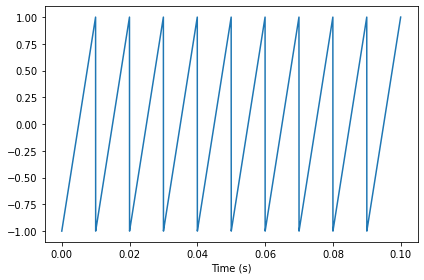
\includegraphics[scale=1]{fig/lab09/lab09_7.png}
		\caption{Пилообразный сигнал}
	\end{center}
\end{figure}

\begin{lstlisting}[language=Python]
spectrum = wave.make_spectrum().integrate().integrate()
spectrum.hs[0] = 0
wave1 = spectrum.make_wave()
wave1.plot()
decorate(xlabel='Time (s)')
\end{lstlisting}
\begin{figure}[H]
	\begin{center}
		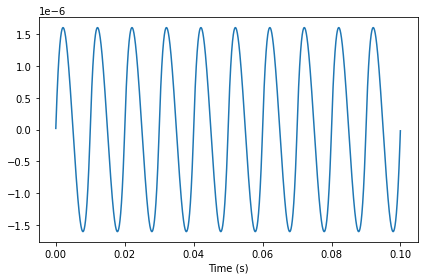
\includegraphics[scale=1]{fig/lab09/lab09_8.png}
		\caption{Изменённый сигнал}
	\end{center}
\end{figure}

Сигнал напоминает синусойду, это связано с фильтрацией низких частот кроме основной.

\begin{lstlisting}[language=Python]
wave.make_spectrum().plot(high=1000)
\end{lstlisting}
\begin{figure}[H]
	\begin{center}
		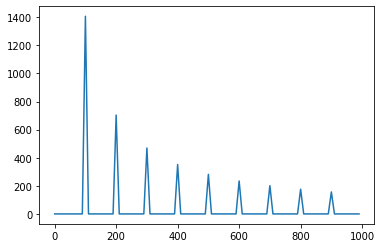
\includegraphics[scale=1]{fig/lab09/lab09_9.png}
		\caption{Спектр исходного сигнала}
	\end{center}
\end{figure}

\begin{lstlisting}[language=Python]
wave1.make_spectrum().plot(high=1000)
\end{lstlisting}
\begin{figure}[H]
	\begin{center}
		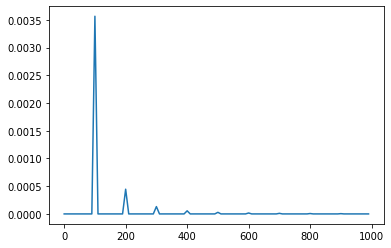
\includegraphics[scale=1]{fig/lab09/lab09_10.png}
		\caption{Спектр нового сигнала}
	\end{center}
\end{figure}


\subsection{Упражнение 4}

Создайте CubicSignal, определённый в thinkdsp. Вычислите вторую разность, дважды применив diff. Как выглядит результат? Вычислите вторую разность, дважды применив differentiate к спектру. Похожи ли результаты? Распечатйте фильтры, соответсвующие второй разнице и второй производной. Сравните их.

Изучим влияние второй разности и второй производной на CubicSignal сигнале.

\begin{lstlisting}[language=Python]
from thinkdsp import CubicSignal
w = CubicSignal(freq=0.0005).make_wave(duration=10000, framerate=1)
w.plot()
\end{lstlisting}
\begin{figure}[H]
	\begin{center}
		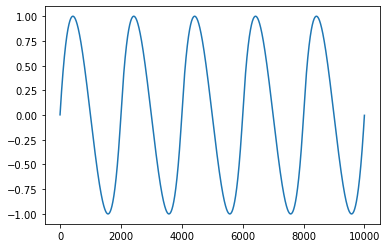
\includegraphics[scale=1]{fig/lab09/lab09_11.png}
		\caption{Кубический сигнал}
	\end{center}
\end{figure}

Первая разность это параболы

\begin{lstlisting}[language=Python]
first = w.diff()
first.plot()
\end{lstlisting}
\begin{figure}[H]
	\begin{center}
		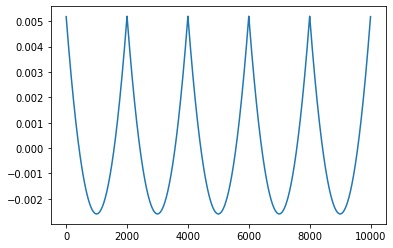
\includegraphics[scale=1]{fig/lab09/lab09_12.png}
		\caption{Первая разность}
	\end{center}
\end{figure}

Вторая разность это пилообразный сигнал.

\begin{lstlisting}[language=Python]
second = first.diff()
second.plot()
\end{lstlisting}
\begin{figure}[H]
	\begin{center}
		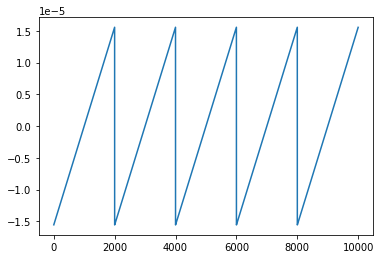
\includegraphics[scale=1]{fig/lab09/lab09_13.png}
		\caption{Вторая разность}
	\end{center}
\end{figure}

Сделаем двойное дифферинцирование.

\begin{lstlisting}[language=Python]
spec = w.make_spectrum().differentiate().differentiate()
third = spec.make_wave()
third.plot()
\end{lstlisting}
\begin{figure}[H]
	\begin{center}
		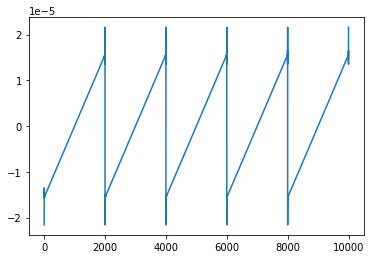
\includegraphics[scale=1]{fig/lab09/lab09_14.png}
		\caption{Полученный сигнал со звоном}
	\end{center}
\end{figure}

В связи с тем что производная не определена в некоторых точках, на графике присутствует звон, используем фильтры:

\begin{lstlisting}[language=Python]
from thinkdsp import zero_pad
from thinkdsp import Wave

diff_window = np.array([-1.0, 2.0, -1.0])
padded = zero_pad(diff_window, len(wave))
diff_wave = Wave(padded, framerate=wave.framerate)
diff_filter = diff_wave.make_spectrum()
diff_filter.plot()
decorate(xlabel='Frequency (Hz)', ylabel='Amplitude ratio')
\end{lstlisting}

\begin{figure}[H]
	\begin{center}
		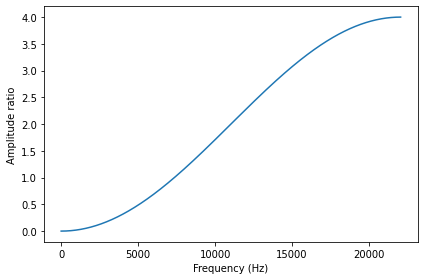
\includegraphics[scale=1]{fig/lab09/lab09_15.png}
		\caption{Полученные фильтры}
	\end{center}
\end{figure}

Для второй производной можно найти соответствующий фильтр, рассчитав фильтр первой прозводной и возведя его в квадрат.
\begin{lstlisting}[language=Python]
deriv_filter = w.make_spectrum()
deriv_filter.hs = (2 * np.pi * 1j * deriv_filter.fs)**2
deriv_filter.plot()
\end{lstlisting}

\begin{figure}[H]
	\begin{center}
		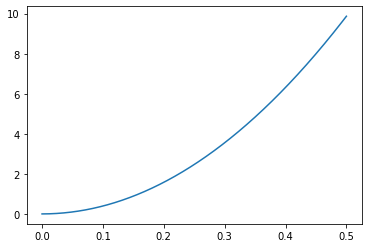
\includegraphics[scale=1]{fig/lab09/lab09_16.png}
		\caption{Полученные фильтры}
	\end{center}
\end{figure}


\subsection{Вывод}

В данной работе были рассмотрены соотношения между окнами во временной области и фильтрами в частотной. Также рассмотрели конечные разности, cumsum - накапливающие суммы с апроксимирующим интегрированием.
